\documentclass[a4paper,11pt]{article}
\usepackage[utf8]{inputenc}
\usepackage{algorithmic}
\usepackage{algorithm}
\usepackage{pst-plot}
\usepackage{graphicx}
\usepackage{endnotes}
\usepackage{graphics}
\usepackage{floatflt}
\usepackage{wrapfig}
\usepackage{amsfonts}
\usepackage{amsmath}
\usepackage{verbatim}
\usepackage{hyperref}
\usepackage{multirow}
\usepackage{pdflscape}

\usepackage{hyperref}
\hypersetup{pdfborder={0 0 0 0}}

\pdfpagewidth 210mm
\pdfpageheight 297mm 
\setlength\topmargin{0mm}
\setlength\headheight{0mm}
\setlength\headsep{0mm}
\setlength\textheight{250mm}	
\setlength\textwidth{159.2mm}
\setlength\oddsidemargin{0mm}
\setlength\evensidemargin{0mm}
\setlength\parindent{7mm}
\setlength\parskip{0mm}

\newenvironment{exercise}[3]{\paragraph{Exercise #1: #2 \textsc{(#3pt)}}\ \\}{
\medskip}
\newcommand{\question}[2]{\setlength\parindent{0mm}\ \\$\mathbf{Q_#1:}$ #2\ \\}

\author{\large{Ilya Kuzovkin, Raul Vicente}}
\title{\huge{Introduction to Computational Neuroscience}\\\LARGE{Practice II: Data Analysis - Continuous Data}}

\begin{document}
\maketitle
\ \\
This is how usual EEG recording of one channel looks like:
\begin{figure}[H]
   \centering
   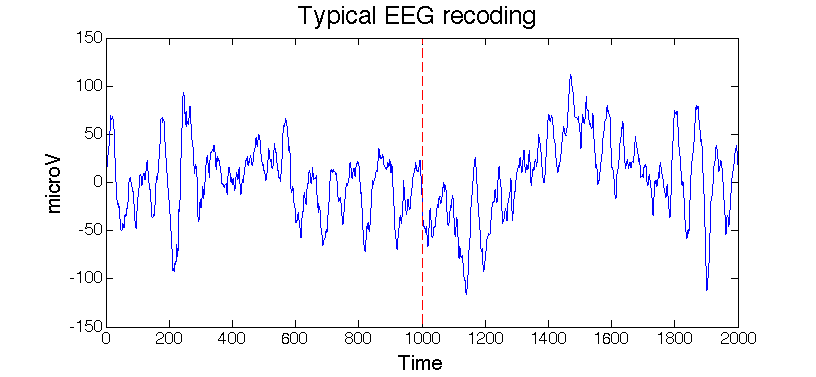
\includegraphics[width=0.8\textwidth]{eegrecording.png} 
\end{figure}
On the $x$ axis there is time, on the $y$ axis strength of the recorded signal in $\mu$V. The dashed line at the time point $x=1000$ is the moment when the \emph{stimulus} (picture) was shown to the test subject.

%
% ERP
%
\begin{exercise}{1}{Event Related Potential (ERP)}{1}
By looking at the plot above one cannot say that showing the stimulus had any considerable effect on the test subject. It seems that there is an increase starting at the time point 1200 and ending at the time point 1500, but that can be a random event, which is not related to the stimulus.

In such studies the way to go is to conduct the same experiment several times and then average the results. In this way the response, if it is there, will reveal itself much more clearly.

In the \texttt{data} folder you have file \texttt{erptrials.csv}. One row is one trial recorded for 2 seconds with sampling rate of 1000 Hz. The stimulus was shown at the time point 1000 (1 second). There are 79 trials in this file. Your task is to plot an average of all 79 trials and see whether there is a clear ERP response or not.
\end{exercise}

%
% Apply fourier
%
\begin{exercise}{2}{Frequency Analysis}{2}
The most popular operation that you can do with continuous brain data is converting it from the \emph{time domain} to the \emph{frequency domain}. Due to the fact that any function can be represented as a sum of sinusoids we can decompose our signal into such sinusoids and observe from which frequency components it consists. In terms of the brain data such transformation makes particular sense, because of the \emph{brain rhythms} -- different frequencies of the firings of the neurons are related to the different kinds of mental activity\footnote{\url{http://en.wikipedia.org/wiki/Electroencephalography\#Wave_patterns}}.

\ \\
In this exercise we will plot \emph{power spectrum} and see how \emph{alpha wave} emerges when the test subject's eyes are closed. In the \texttt{data} folder you can find two files: \texttt{eyes\_open.csv} and \texttt{eyes\_closed.csv}. The data is recorded from the channel \texttt{Pz}. One row contains 4 seconds of the signal, sampling rate is 512. Each file has 15 recordings.

\ \\
Your task is to perform Fourier analysis on both datasets, plot power spectra and compare the results. Do it as follows:
\begin{enumerate}
	\item Plot some of the signals just to see how they look like.
	\item For each recorded signal (2048 data points):
		\begin{enumerate}
			\item Use \texttt{fft(signal)} to compute power spectrum of this signal. You will get a vector of complex numbers.
			\item Use \texttt{abs(result\_of\_fft)} to obtain the magnitude\footnote{\url{http://www.mathworks.se/help/matlab/ref/abs.html}}. \texttt{abs(result\_of\_fft)}$^2$ will give you power.
		\end{enumerate}
	\item Sum together 15 power spectrum distributions, that you got from the previous step.
	\item And divide the resulting vector by 15 to obtain the average.
	\item Plot it. You will see that the right part of the graph is mirror image of the left part. Discard the right part.
	\item Your $x$ axis goes from 1 to 1024, which does not correspond to actual frequencies. Compute correct $x$ axis as follows:
		\begin{verbatim}
		dt = 1/512;             % time step
df = 1/4;               % frequency step
fNQ = 1/dt/2;           % fNQ is the maximal frequency, in our case it is 256
                        %   if you have discarded part of the data in step 5 
                        %   or 512 if you did not
xaxis = (0:df:fNQ-df);  % points for your X axis, should be of the same length 
                        %   as the vector of frequencies
		\end{verbatim}
	\item And plot it again
		\begin{verbatim}
		plot(xaxis, powers_average);
		\end{verbatim}
		Now your axis goes from 0 to 256 (or 512) with step of 4, which corresponds to the frequency range \texttt{pow} function produced.
\end{enumerate}

\ \\
After making the plot more beautiful and focusing on the range from 0 to 30 Hz you should obtain the result that looks something like this:
\begin{figure}[H]
   \centering
   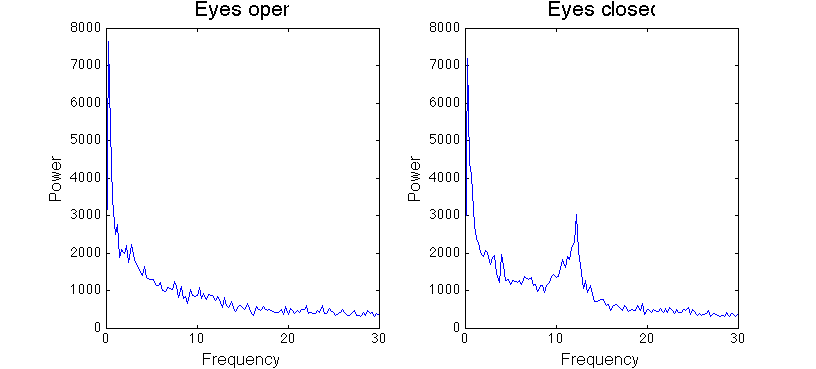
\includegraphics[width=1\textwidth]{fouriereyes.png} 
\end{figure}
\end{exercise}


%
% Epilepsy
%
\begin{exercise}{3}{Epilepsy}{2}
In the folder \texttt{data/epilepsy} you have two data files: \texttt{sz4\_pre.dat} and \texttt{sz4\_ict.dat}. This data was recorded using ECoG\footnote{http://en.wikipedia.org/wiki/Electrocorticography} array. The file with the suffix \texttt{\_pre} is recorded before the seizure and the \texttt{\_ict} file is recorded during the epilepsy seizure. Read the \texttt{README.txt} file for the description of the data. Your task is to perform Fourier analysis on both files and see how brain activity changes during the epilepsy seizure. Speculate what is the nature of the peak around 60Hz.
\paragraph{Hint.} Reuse the code from the previous exercise.
\paragraph{Hint.} The data has readings from the 76 electrodes. First make Fourier transform on each of them separately, then compute the power spectra (each one separately) and then compute the average and plot that.
\end{exercise}



%
% Discuss
%
\begin{exercise}{4}{Nyquist theorem}{1}
What does Nyquist theorem say? What does it mean? What are the implications?\\
What does this picture illustrate?
\begin{figure}[H]
   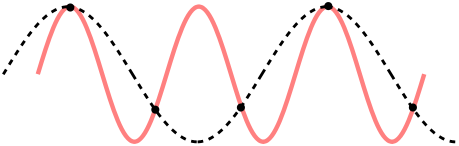
\includegraphics[width=0.4\textwidth]{nyquist.png} 
\end{figure}
\ \\
Prepare to present and explain the theorem to your fellow students.
\end{exercise}


%
% Play DFT
%
\begin{exercise}{5*}{Discrete Fourier Transform (DFT)}{bonus 2}
Now let us have a look on what happens behind the scenes when you call the \texttt{fft}\footnote{Actually Fast Fourier Transform (FFT) is a specific algorithm. In this exercise we do not analyse that, but rather look at the equations, which FFT solves in his own mysterious way.} function. Fourier transform is possible because, as we mentioned before, any function can be represented as a sum of sinusoidal functions of different frequencies and amplitudes. If you have some variable changing over time you can transform this data from the \emph{time domain} (time on the $x$ axis and the value of the variable on the $y$ axis) to the \emph{frequency domain} (frequency on the $x$ axis and it's \emph{power} on the $y$ axis) to see if there is any periodicity in the changes of that variable.

\ \\
Transformation is defined both for continuous and discrete data. On practice we mostly work with a discrete signal and therefore we use Discrete Fourier Transform (DFT). The equation for the discrete transform is
$$X_f = \displaystyle\sum_{t=0}^{N-1}x_t e^{-i2\pi f\frac{t}{N}}$$
where
\begin{itemize}
\itemsep 0em
	\item $f$ is the frequency of the component, contribution of which you are trying to estimate.
	\item $X_f$ is a complex number, that encodes both amplitude and phase of the sinusoidal component.
	\item $x_t$ is a value of your signal at the time point $t$.
	\item $N$ is the total number of time points.
\end{itemize}
Let us say that you would like to know contribution of sinusoidal components of frequencies from 1 to 100 Hz. Then you should apply this equation 100 times. As a result you will get 100 complex numbers.
To extract amplitude from these numbers use the following equation on each of them:
$$A_f = 2\frac{\sqrt{\text{Re}(X_f)^2 + \text{Im}(X_f)^2}}{N}$$
Now you have all the contributions and you have completed Discrete Fourier Transform of your signal. For example if 7th number is "25" then it means that the amplitude of the sinusoidal component with frequency 7 $\times$ df Hz is 25.

\ \\
Here you see a curve, that is a sum of three sinusoids. Your task is to apply DFT and find out frequencies and amplitudes of those components. You can find data points for this curve in the file \texttt{curve.csv}.
\begin{figure}[htbp]
   \centering
   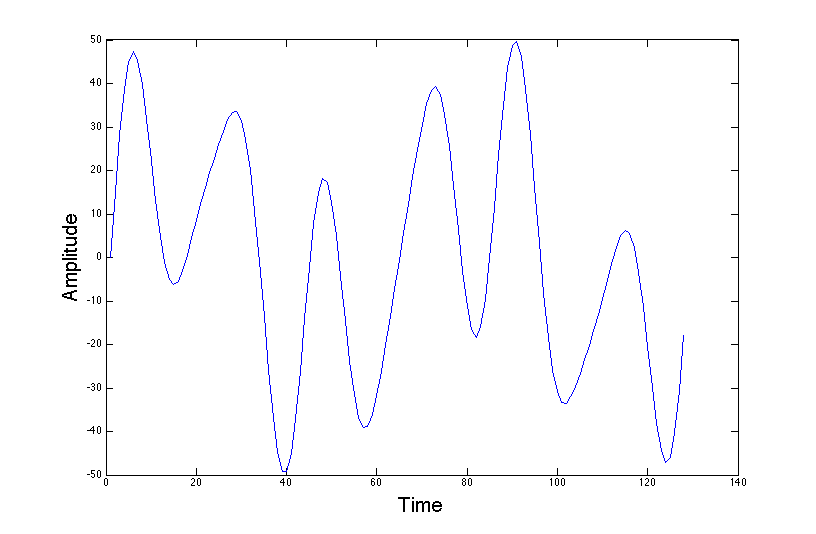
\includegraphics[width=0.6\textwidth]{dodft.png} 
\end{figure}
\end{exercise}

\ \\
\ \\
\ \\
\ \\
Please submit a \texttt{pdf} report with the answers to the questions, plots and comments about your solutions. Also submit the code for the programming exercise(s). Pack those into the \texttt{zip} archive and upload to the course web page.

\end{document}










